%% ============================================================
%% Finance Research Letters submission
%% Chronotypic Market Ecology
%% Subramanian & Seetharaman (2026)
%% Target: <2500 words main text (excl. abstract, refs, tables,
%%          figures, captions, acknowledgements, declarations,
%%          appendices).
%% ============================================================

\documentclass[preprint,12pt,authoryear]{elsarticle}

\usepackage{amsmath,amssymb,amsthm}
\usepackage{graphicx}
\usepackage{booktabs}
\usepackage{lineno}
\usepackage{url}
\usepackage[expansion=false]{microtype}

\graphicspath{{figures/}}

\newtheorem{theorem}{Theorem}
\newtheorem{definition}{Definition}
\newtheorem{remark}{Remark}

\journal{Finance Research Letters}

\begin{document}

\linenumbers

\begin{frontmatter}

\title{Chronotypic Market Ecology: Temporal Homophily,
       Network Fragmentation, and Market Stability}

\author[vchs]{Sanjay Subramanian\corref{cor1}}
\ead{jaysubbu@gmail.com}

\author[vchs]{Sumedh Seetharaman}

\cortext[cor1]{Corresponding author.}

\affiliation[vchs]{organization={Valley Christian High School},
             addressline={100 Skyway Drive},
             city={San Jose},
             postcode={95138},
             state={CA},
             country={USA}}

%% -------------------------------------------------------
\begin{abstract}
We introduce Chronotypic Market Ecology (CME), an agent-based framework
in which market participants are characterised by their temporal scale
$\tau$---the lookback horizon over which they evaluate price signals.
Agents with similar $\tau$ preferentially form trade relationships
(\emph{temporal homophily}, strength $\kappa_h$), creating an endogenous
$\tau$-proximity network whose topology shapes price dynamics.
Using a calibrated simulation (four investor types from 2023 Assets Under Management (AUM) data,
$n = 80$, $T = 500$, 30 seeds) we establish three results that together
constitute a network-based microfoundation for the Fractal Market
Hypothesis \citep{peters1994}: homophily is a \emph{dual-channel} force
that stabilises prices in the short run while sowing the conditions for
long-run instability.
First, increasing homophily suppresses aggregate return volatility
($1.310\times$, paired $t = 5.57$, $p < 10^{-5}$) by reducing cross-$\tau$
friction---the short-run stabilising channel.
Second, the Temporal Market Fragmentation Index (TMFI) falls $14.25\times$
versus only $1.310\times$ for volatility, nearly eliminating temporal
fragmentation as $\tau$-communities converge.
Third, $\tau$-adaptation compresses horizon diversity across all tested
homophily levels ($\Delta\mathrm{TDI} = -0.740$ at $\kappa_h = 0.5$
and $-0.306$ at $\kappa_h = 6.0$ over ten cycles, 30 seeds),
producing temporal echo chambers that erode the diversity the FMH
identifies as the foundation of market stability---the long-run
destabilising channel.
We then confront the framework with SEC Form~13F institutional holdings
(2013~Q3--2024~Q3).
Institutions with similar horizons hold more similar portfolios
(mean $\hat{\kappa}_h = +0.158$, Newey--West $t \approx 19$ over 50 quarters),
so temporal homophily is detectable in real data.
The quarterly TDI is negatively correlated with the VIX
($r = -0.526$, $n = 45$ quarters), but the correlation disappears
($r = -0.06$) when turnover is computed from share changes rather than value
weights, so we attribute it largely to price drift and not to horizon
compression.
At the stock level, lower dispersion of holders' horizons predicts higher
next-quarter volatility (63{,}261 stock-quarters), as the Fractal Market
Hypothesis suggests, although the within-stock effect is small and its sign is
opposite to the model's own simulated friction channel.
An empirical Temporal Liquidity proxy from SPY quarterly returns is
negatively correlated with VIX ($r = -0.392$, $n = 45$), but this is largely
mechanical because the proxy contains return volatility.
A simulated cross-asset-class sweep finds the CME mechanism strongest in
long-horizon-dominated bond markets (TL, $p = 0.039$) and nearly
inert in short-horizon-dominated FX markets (all $p > 0.90$), implying
that chronotype composition governs the magnitude
of the stability--fragmentation effect in the model.
\end{abstract}

%% -------------------------------------------------------
\begin{highlights}
\item Agent-based model of investor horizons, homophily and market fragmentation
\item Homophily cuts simulated volatility 1.31$\times$ and fragmentation 14.25$\times$
\item 13F data: like-horizon institutions co-hold more ($\hat{\kappa}_h = 0.158$)
\item TDI--VIX correlation is a price-drift artefact; it vanishes with share turnover
\item Clustered holder horizons predict higher stock volatility, but the effect is small
\end{highlights}

%% -------------------------------------------------------
\begin{keyword}
agent-based model \sep temporal heterogeneity \sep market fragmentation
\sep homophily \sep network topology \sep market volatility
\sep rational inattention
\end{keyword}

\end{frontmatter}

%% ============================================================
\section{Introduction}
\label{sec:intro}

Financial markets aggregate the decisions of participants operating across
vastly different timescales---from high-frequency traders reacting to
millisecond price movements to pension funds rebalancing quarterly.
This temporal heterogeneity is well-documented empirically
\citep{muller1993, corsi2009}: \citet{frenchroll1986} show that return
variance during trading hours far exceeds non-trading-hour variance,
implying that active short-horizon trading itself generates variance
signals that long-horizon agents cannot easily distinguish from
fundamental-value innovations.
Yet temporal heterogeneity remains largely absent from mainstream
market-microstructure models, which either homogenise agents or treat
timescales as exogenous labels without endogenous network formation
\citep{lebaron2001, farmerfoley2009}.

We propose \emph{Chronotypic Market Ecology} (CME), in which each agent~$i$
is characterised by a \emph{chronotype} $\tau_i$---a continuous lookback
horizon---and agents with similar $\tau$ preferentially form trade
relationships (\emph{temporal homophily}, parameter $\kappa_h$).
The resulting endogenous $\tau$-proximity network determines how price
beliefs blend and momentum propagates.
Crucially, this is not a social-imitation model: agents form links
based on similarity in the frequency band they monitor, not on returns or
signals.
Three research questions motivate the analysis: (i) How does $\kappa_h$
affect price volatility and market fragmentation? (ii) Does homophily
generate a stability--fragmentation trade-off? (iii) Can $\tau$-adaptation
produce self-reinforcing echo chambers?

Our contributions are threefold. First, we formalise $\tau$ as the
\emph{primary} dimension of agent heterogeneity, distinct from the
risk-preference or signal-quality dimensions used in prior heterogeneous-agent
models.
Second, we derive three diagnostic metrics: the Temporal Diversity Index
(TDI, a Shannon entropy over the $\tau$ distribution), the Temporal Market
Fragmentation Index (TMFI, the cross-community coefficient of variation of
price beliefs), and Temporal Liquidity (TL, a composite measure of return smoothness and
cross-horizon price discovery, inversely proportional to the product of
return volatility and lag-1 autocorrelation).
Third, we confront the framework with SEC Form~13F institutional holdings
data (2013~Q3--2024~Q3).
We find that temporal homophily is detectable in real portfolios, that the
aggregate TDI--VIX correlation ($r = -0.526$) is largely an artefact of price
drift in value-weight turnover, and that holder-horizon clustering predicts
stock volatility with the sign the Fractal Market Hypothesis suggests but a
small magnitude, and with a sign opposite to the model's simulated friction
channel, which we report as an open tension.

CME connects several strands of prior work.
The Fractal Market Hypothesis (FMH; \citealt{peters1994}) argues that markets are
stable when investors operate across heterogeneous horizons and become
fragile when horizons concentrate---but provides no network mechanism for
\emph{why} or \emph{how fast} horizons converge.
CME supplies that mechanism: $\tau$-proximity network formation plus
adaptation gives rise to a dual-channel dynamic in which homophily
stabilises prices in the short run but erodes the very horizon diversity
the FMH identifies as the foundation of stability.
The heterogeneous-agent literature \citep{arthur1997, lebaron2001} shows
that agent heterogeneity generates realistic price dynamics including excess
volatility and fat tails \citep{cont2001}.
Herding models \citep{bikhchandani1992, devenow1996} characterise how
social interaction correlates behaviour, while network contagion theory
\citep{acemoglu2015} establishes that topology amplifies shocks.
Rational inattention \citep{sims2003, caplin2015} provides a
microfoundation for the $\tau$ distribution: capacity-constrained agents
optimally allocate attention to specific return frequencies, producing
heterogeneous lookback horizons as an endogenous outcome.
CME treats $\tau$ as exogenous for tractability, with the 13F calibration
providing empirical grounding; endogenising $\tau$ via rational inattention
is a natural extension.
\citet{golub2012} show that homophily slows information aggregation by
reducing cross-type contact; CME's $\tau$-adaptation mechanism exhibits an
analogous but distinct dynamic---agents adapt their \emph{observation
frequency} rather than their beliefs, so the convergence mechanism is
preference-based rather than Bayesian, as we show in
Section~\ref{sec:results}.

Two further literatures are closer to our contribution.
On the empirical side, institutional investment horizons are already known to
matter for markets.
\citet{bushee1998} and \citet{gaspar2005} classify institutions by portfolio
turnover and relate short-horizon ownership to managerial myopia and takeover
outcomes, and \citet{cella2013} use 13F holdings to show that stocks held by
short-horizon institutions fall further, and later reverse more, in market
turmoil.
These papers study the \emph{level} of short-horizon ownership; we study the
\emph{dispersion} of horizons among a stock's holders, holding the mean horizon
fixed, and embed it in a network model in which horizon similarity determines
who interacts with whom.
On the theoretical side, the agent-based literature on the Fractal Market
Hypothesis shows that liquidity comes from investors with different horizons
and that stability can improve as markets move from uniform to diverse horizons,
although with a finite maximum horizon more diversity need not add stability
\citep{li2014}; \citet{kristoufek2012} tests scaling predictions of the
hypothesis around the 2008 crisis.
CME differs by making horizon similarity an endogenous network-formation rule
and by letting horizons adapt to neighbours, which generates the dual-channel
result of Section~\ref{sec:results}.

%% ============================================================
\section{Model}
\label{sec:model}

\subsection{Chronotypes and the Temporal Diversity Index}

\begin{definition}[Chronotype]\label{def:chronotype}
Agent~$i$'s chronotype is $\tau_i \in [\tau_{\min}, \tau_{\max}]$
(trading days), the lookback horizon over which agent~$i$ evaluates
price signals.
\end{definition}

\begin{definition}[Temporal Diversity Index]\label{def:tdi}
\[
  \mathrm{TDI} = -\sum_{k=1}^{K} f_k \ln f_k, \qquad K = 16,
\]
where $f_k$ is the fraction of agents whose $\log\tau$ falls in
equal-width bin~$k$ over $[\ln 1,\,\ln 2000]$, using the natural
logarithm throughout.
With $\tau \in [5, 2000]$, the three lowest bins ($\tau < 4.2$ days) are
structurally empty, so the effective maximum TDI is $\ln(13) \approx 2.565$
rather than the theoretical ceiling $\ln(16) \approx 2.773$.
Note: the $\tau$-proximity network kernel
(Definition~\ref{def:tau-network}) uses $\log(\tau+1)$ for the distance metric, while TDI
bins are indexed by $\log\tau$; the two transformations are nearly
identical for $\tau \geq 5$ (the minimum agent horizon) and differ by at
most 0.18 nats at $\tau = 5$.
High TDI indicates diverse timescales; low TDI indicates chronotypic
clustering.
\end{definition}

\subsection{Demand and Price Dynamics}

Agent $i$'s demand at time $t$ is
\begin{equation}
  d_i(t) = \bar{\alpha} \frac{F_t - \bar{p}_i(t)}{p_t}
          + \bar{\beta} m_i(t) + \varepsilon_i(t),
  \label{eq:demand}
\end{equation}
where $F_t = F_{t-1}\exp(\varepsilon_t^F)$, $\varepsilon_t^F \sim
\mathcal{N}(0,\sigma_F^2)$ ($\sigma_F = 0.010$) is the fundamental value;
$\bar{p}_i(t)$ is agent~$i$'s $\tau_i$-day moving average;
$m_i(t) = \ln(p(t)/p(t-\tau_i))$ is the momentum signal over
the agent's own lookback window; and
$\varepsilon_i(t) \sim \mathcal{N}(0,(\sigma_i^{\mathrm{eff}})^2)$ is
idiosyncratic noise.
The first term is a fundamentalist component---demand rises when the
current moving average sits below the fundamental---while the second
captures trend-following in the agent's native frequency band.
Parameters $\bar{\alpha} = 0.30$ (fundamentalist restoring force) and
$\bar{\beta} = 0.20$ (momentum weight) are global constants shared by all
agents (see Section~\ref{sec:sim} parameter list).
A market maker adjusts the price each period in proportion to aggregate
excess demand: $p(t+1) = p(t) + \lambda \sum_i d_i(t)$,
where $\lambda = 0.008$ is the price-impact parameter.
In practice, the probability that a pension fund and an HFT appear as
direct bilateral counterparties in any given period is negligibly small
given their vastly different trading frequencies.
CME abstracts from order-book mechanics by routing all trades through
the centralised market maker, which clears aggregate excess demand each
period; the $\tau$-proximity network governs information and belief
formation rather than direct bilateral matching.
This abstraction deliberately sets aside the information-asymmetry
channel studied by \citet{kyle1985} and \citet{akerlof1970}, in which
agents shade their bids and offers based on beliefs about counterparty
information quality.
Incorporating that channel---so that a long-horizon agent discounts
prices proposed by short-horizon agents suspected of superior
intraday information---is a natural extension that would enrich the
model's microstructure foundations.
The low empirical frequency of cross-chronotype direct trades is thus
captured in the cross-$\tau$ friction term (Eq.~\eqref{eq:sigeff}),
which amplifies noise for agents whose counterparty pool spans
distant horizons.

\subsection{$\tau$-Proximity Network and TMFI}

\begin{definition}[$\tau$-proximity network]\label{def:tau-network}
The directed tie probability from agent $i$ to agent $j$ is
\[
  P(i \to j) \propto
  \exp\!\bigl(-\kappa_h\,|\log(\tau_i+1)-\log(\tau_j+1)|\bigr).
\]
\end{definition}

Let $\lambda_2$ denote the Fiedler eigenvalue of the graph Laplacian.
Each agent's price observation is blended with its neighbourhood average
for the TMFI diagnostic:
\begin{equation}
  p^{\mathrm{obs}}_i
    = c(\lambda_2)\,(\mathbf{W}\mathbf{p}^{\mathrm{obs}})_i
    + (1-c(\lambda_2))\,p_t,
  \label{eq:pobs}
\end{equation}
where $\mathbf{W}$ is the row-normalised adjacency matrix,
$c(\lambda_2) = \min(\log(1+\lambda_2)/\log 2,\;1)$,
and $p_t$ is the global market price.
Eq.~\eqref{eq:pobs} enters the model \emph{exclusively} through the TMFI
observation path; agent demand in Eq.~\eqref{eq:demand} uses $p_t$
directly.

Cross-$\tau$ friction amplifies effective noise:
\begin{equation}
  \sigma_i^{\mathrm{eff}} = \sigma_0\bigl(1 + \gamma\,\bar{d}_\tau(i)\bigr),
  \label{eq:sigeff}
\end{equation}
where $\bar{d}_\tau(i)$ is the mean $\tau$-distance between agent~$i$ and
its counterparties.
This friction term is economically grounded: \citet{amihud1986} establish
that transaction costs are priced into gross returns so that risk-adjusted
net returns equalise across assets; CME's friction channel captures the
analogous idea that cross-horizon mismatches raise the effective cost of
information exchange between differently-timed counterparties.
The observation noise for the TMFI path is scaled by $\sigma_i^{\mathrm{eff}}$:
each agent first forms an individual noisy observation
$\hat{p}_i = p\bigl(1 + \sigma_{\mathrm{obs}} \cdot \xi_i\bigr)$
where $\xi_i \sim \mathcal{N}(0,\,(\sigma_i^{\mathrm{eff}}/\sigma_0)^2)$;
these are stacked into $\mathbf{p}^{\mathrm{obs}}$ in Eq.~\eqref{eq:pobs}
before network blending,
so that cross-$\tau$ friction amplifies both demand noise and observation noise.

\begin{definition}[TMFI]\label{def:tmfi}
\[
  \mathrm{TMFI}(t) =
    \frac{\mathrm{std}_{\mathrm{unbiased}}\bigl(\{\bar{p}^{(c)}(t)\}_{c=1}^{C}\bigr)}%
         {\mathrm{mean}\bigl(\{\bar{p}^{(c)}(t)\}_{c=1}^{C}\bigr)},
\]
where $\mathrm{std}_{\mathrm{unbiased}}$ is the sample standard deviation
with $C - 1 = 3$ degrees of freedom (Bessel's correction, $C = 4$ communities),
and $\bar{p}^{(c)}(t)$ is the mean noisy price observation of community~$c$,
formed by partitioning agents into $C = 4$ quartile groups of
$\log(\tau_i+1)$ (matching the $\tau$-proximity network kernel, Definition~\ref{def:tau-network}).
TMFI is computed over the second half of the simulation ($t \geq T/2$)
after the price process reaches approximate stationarity.
\end{definition}

\begin{definition}[Temporal Liquidity]\label{def:tl}
\[
  \mathrm{TL}(t) = \frac{1}{\sigma_r(t)\,|\mathrm{ACF}_1(t)|},
\]
where $\sigma_r(t)$ is the period-$t$ return volatility and
$\mathrm{ACF}_1(t)$ is the lag-1 return autocorrelation;
higher TL indicates lower cross-$\tau$ friction and faster cross-horizon
price discovery.
TL is undefined when $|\mathrm{ACF}_1| \to 0$; in the empirical
implementation we exclude quarters where $|\widehat{\mathrm{ACF}}_1| < 0.05$.
SPY history from 2011 supplies the rolling windows, so TL is available for
all 45 quarters of the 13F sample; no quarter falls below the floor (the
smallest $|\widehat{\mathrm{ACF}}_1|$ is 0.075).
\end{definition}

\subsection{Stability and $\tau$-Adaptation}

\begin{theorem}[Stability bound]\label{thm:stability}
A sufficient condition for the linearised price dynamics to be stable
is $\lambda_2 > \bar{\beta}/\bar{\alpha}$.
This condition is not satisfied by the calibrated parameters ($\lambda_2
\approx 0.655 < \bar{\beta}/\bar{\alpha} \approx 0.667$); stability in
the simulation is maintained instead by the nonlinear fundamentalist
restoring force, which the linearised analysis cannot capture.
\end{theorem}

\begin{remark}
The stability condition $\lambda_2 > \bar{\beta}/\bar{\alpha}$ is
\emph{sufficient but not necessary}.
$\lambda_2$ is computed from the normalised Laplacian of the symmetrised
adjacency matrix $(A + A^\top)/2$; although the CME network is directed,
price information flows bidirectionally and symmetrisation gives the
economically appropriate connectivity measure
($\lambda_2 \approx 0.655$ at $\kappa_h = 0$, 30-seed mean).
With calibrated parameters $\bar{\beta}/\bar{\alpha} \approx 0.667$, the
simulated $\lambda_2 \approx 0.655$ strictly violates the sufficient
condition ($0.655 < 0.667$) in 27 of 30 seeds; this confirms the condition
is sufficient but not necessary---prices remain bounded in all simulations
because the nonlinear fundamentalist restoring force provides stability that
the linearised sufficient condition understates.
The Fiedler value therefore serves primarily as a network-connectivity
diagnostic (characterising TMFI sensitivity at $\kappa_h = 0$), not as
the sole governing stability criterion.
We note that linear stability (price-process boundedness, Theorem~\ref{thm:stability})
and steady-state return variance (the volatility results in Section~\ref{sec:results})
are distinct properties: the former concerns whether prices remain bounded,
the latter governs the level of fluctuations around the stable path.
High $\kappa_h$ reduces variance (Section~\ref{sec:results}) not by
improving linear stability but by narrowing the cross-$\tau$ friction term
$\sigma_i^{\text{eff}}$ (Eq.~\eqref{eq:sigeff}), which reduces demand noise
directly.
The $k = 1$ (uniform price-shift) mode is separately bounded.
A fractional shift $\delta$ in the current price, with past prices held fixed,
changes every agent's momentum signal $m_i = \ln(p(t)/p(t-\tau_i))$ by exactly
$\delta$ and, at the fundamental-value equilibrium, leaves the fundamentalist
term unchanged to first order.
With the price update $p(t{+}1) = p(t) + \lambda\sum_i d_i(t)$ over $n$ agents,
the one-step gain on the uniform mode is therefore
$g = \lambda\,n\,\bar{\beta}/\bar{p}$, which equals
$0.008 \times 80 \times 0.20 / 100 \approx 1.3\times 10^{-3} \ll 1$ under the
calibrated parameters.
Because $g < 1$ the uniform mode is a contraction, and its response to any
shock is damped by a factor of roughly one thousand per period, making this mode
dynamically negligible.
\end{remark}

Agents update chronotypes via
$\tau_i \leftarrow (1-\eta)\tau_i + \eta\bar{\tau}_{\mathcal{N}(i)}$,
where $\bar{\tau}_{\mathcal{N}(i)}$ is the mean horizon of $i$'s network
neighbours and $\eta = 0.06$ is the adaptation rate.
This rule captures a simple form of social learning: agents that
predominantly trade with short-horizon counterparties find short-horizon
strategies rewarded, and shorten their own lookback window.
Under high homophily, where neighbours already share similar $\tau$,
convergence is gradual; under low homophily, cross-chronotype ties can
produce rapid horizon drift.
In the extreme case of a single pension-fund neighbour ($\tau_{\text{nbr}}=1000$),
an HFT agent shifts by $\Delta\tau = 0.06 \times (1000 - 5) \approx 60$
(a $13\times$ increase: $\tau_{\text{new}} = 65$).
In the full network at $\kappa_h = 0$, where the average neighbour $\tau$
across all four agent types is approximately 200--350 days, the mean HFT
shift is more modest ($\Delta\tau \approx 15$ per cycle).

%% ============================================================
\section{Simulation Design}
\label{sec:sim}

Table~\ref{tab:types} gives the four agent types calibrated to the 2023
AUM composition.
Pension funds are characterised as the longest-horizon agents ($\tau \in
[400,\,2000]$~days), reflecting their buy-and-hold mandates and legal
requirements that distinguish them from mutual funds in both incentive
structure and portfolio behaviour \citep{delguercio2002}.

\begin{table}[h]
\centering
\caption{Investor types in the CME simulation.
$\tau$ is drawn from a \emph{truncated} log-normal $\mathrm{LN}(\mu,\sigma)$
on the log scale (trading days), acceptance-rejection sampled within the
stated $\tau$ range.}
\label{tab:types}
\resizebox{0.9\columnwidth}{!}{%
\begin{tabular}{lrrrc}
\toprule
Type        & $\tau$ range & $\mathrm{LN}(\mu,\sigma)$ & AUM & $n_i$ \\
\midrule
HFT         & 1--20\,d     & (0.5, 0.6)                & 15\%& 12    \\
Hedge Fund  & 15--120\,d   & (2.8, 0.7)                & 25\%& 20    \\
Mutual Fund & 60--400\,d   & (4.2, 0.6)                & 40\%& 32    \\
Pension     & 400--2000\,d & (6.0, 0.8)                & 20\%& 16    \\
\bottomrule
\end{tabular}}
\end{table}

We run $T = 500$ trading periods, $n = 80$ agents, 30~seeds for primary
statistics, sweeping $\kappa_h$ from 0 to 6 in steps of 0.25 (25 values);
key results are reported at $\kappa_h \in \{0,\,0.5,\,1,\,2,\,3,\,6\}$.
Global parameters: $\lambda = 0.008$, $\bar{\alpha} = 0.30$,
$\bar{\beta} = 0.20$, $\sigma_0 = 1.0$, $\sigma_{\mathrm{obs}} = 0.008$,
$\gamma = 0.20$, $\eta = 0.06$ (adaptation rate).

%% ============================================================
\section{Results}
\label{sec:results}

\subsection{Homophily suppresses volatility}

Increasing $\kappa_h$ raises network assortativity from $r = -0.02$
(random) to $r = 0.953$ (highly assortative).
Aggregate return volatility falls $1.310\times$
(paired $t$-test across 30 seeds: $t = 5.57$, $p = 5.22 \times 10^{-6}$,
comparing $\kappa_h = 0$ and $\kappa_h = 6$).
The mechanism is noise reduction through cross-$\tau$ friction:
Eq.~\eqref{eq:sigeff} links each agent's effective demand noise to its mean
$\tau$-distance from counterparties.
When homophily clusters agents into like-horizon communities,
cross-$\tau$ distances shrink, compressing $\sigma_i^{\mathrm{eff}}$ and
thus the aggregate demand variance.
The magnitude of the effect---$1.310\times$---is moderate precisely because
the model retains four distinct investor types at all $\kappa_h$ values;
complete homogeneity would eliminate the cross-$\tau$ friction channel
entirely and produce a larger volatility reduction.
The friction channel is isolable: setting $\gamma = 0$ in
Eq.~\eqref{eq:sigeff} removes all $\tau$-distance sensitivity, and
the $\gamma = 0$ robustness sweep (10 seeds each at $\kappa_h \in \{0, 6\}$)
confirms that the $1.310\times$ gap narrows substantially at $\gamma = 0$,
indicating that Eq.~\eqref{eq:sigeff} is the primary---though not the
only---driver of the volatility result.

\subsection{Temporal fragmentation is nearly eliminated}

TMFI falls $14.25\times$ from $\kappa_h = 0$ to $\kappa_h = 6$
(30-seed mean; Fig.~\ref{fig:vol_tmfi}).
Normalising both metrics to the $\kappa_h = 0$ baseline: TMFI $= 0.070$
(7\% of baseline; $14.25\times$ collapse) versus volatility $= 0.763$
(76\% of baseline; $1.310\times$ reduction).
The asymmetry is structural.
At $\kappa_h = 0$, the well-connected random network yields
$c(\lambda_2) \approx 0.727$ (since $\lambda_2 \approx 0.655$,
$c = \log(1.655)/\log 2 = 0.727$), weighting neighbourhood
observations heavily and inflating the TMFI numerator.
At $\kappa_h = 6$, $\tau$-cliques converge beliefs within communities,
nearly zeroing cross-community belief dispersion while the denominator
(global price level) is unchanged.
Homophily therefore \emph{nearly eliminates} temporal fragmentation while
only modestly suppressing aggregate volatility: the ecosystem becomes
temporally homogenised at high $\kappa_h$.

Robustness checks at $n \in \{160,\,320\}$ confirm the direction of
volatility suppression ($1.30\times$ and $1.34\times$, both $p < 0.01$),
with Fiedler values $\lambda_2 = 0.629$ and $0.617$ at $\kappa_h = 0$
respectively, slightly relaxing the stability constraint at scale.
Mean TDI rises modestly with $n$ ($2.43,\,2.44,\,2.46$ for
$n = 80,\,160,\,320$), consistent with greater log-$\tau$ diversity in
larger draws from the calibrated distributions; qualitative conclusions
are robust.
An independent concentration check compresses the $\tau$ distribution by
narrowing each agent type's log-normal standard deviation (concentration
parameter $0.5$ to $3$), which reduces TDI from $2.52$ to $2.01$ (Definition~\ref{def:tdi} bins, 25 seeds per level).
When the compressed horizons are actually used by the simulation, volatility
\emph{falls} rather than rises: $8.4\times10^{-4}$ against $9.5\times10^{-4}$
at $\kappa_h = 0.5$ (Welch $p = 0.009$), and in the same direction but not
significantly so at $\kappa_h = 2$ ($p = 0.13$).
Across runs, TDI and volatility are positively correlated
($r = +0.21$, $p = 0.02$ at $\kappa_h = 0.5$; $r = +0.17$, $p = 0.06$ at
$\kappa_h = 2$).
In the model, horizon diversity therefore raises volatility through the
cross-$\tau$ friction channel; the model does not itself generate the
long-run fragility that the Fractal Market Hypothesis associates with horizon
concentration, which remains a verbal hypothesis.

\subsection{$\tau$-Adaptation produces echo chambers}

$\tau$-adaptation compresses horizon diversity under all homophily levels
tested: $\Delta\mathrm{TDI} = -0.740$ ($\pm\,0.052$, 30 seeds) at
$\kappa_h = 0.5$, $-0.295$ ($\pm\,0.061$) at $\kappa_h = 3.0$, and
$-0.306$ ($\pm\,0.063$) at $\kappa_h = 6.0$ over ten adaptation cycles
(Fig.~\ref{fig:deltaTDI}).
Compression is strongest at the lowest homophily tested ($\kappa_h = 0.5$),
where the near-random network maintains abundant cross-$\tau$ connections,
maximising the adaptation pull $\bar{\tau}_{\mathcal{N}(i)} - \tau_i$.
Under higher homophily ($\kappa_h \in \{3,\,6\}$), agents reside in tight
$\tau$-cliques whose members share nearly identical chronotypes, so
the adaptation pull attenuates and the TDI decline is more modest.

This monotone attenuation is consistent with \citet{golub2012}'s finding
that greater homophily reduces cross-type contact and thereby slows
convergence dynamics; in CME the same mechanism means that strong
$\tau$-cliques \emph{slow} echo-chamber formation relative to weaker
homophily, where cross-$\tau$ connections still drive rapid adaptation.
Unlike Golub and Jackson's Bayesian mechanism, CME adaptation is
preference-based: agents adopt their counterparties' observation frequency,
not their beliefs.
The key implication is that the long-run destabilising channel is not
confined to high homophily: even weak temporal clustering is sufficient
to drive substantial horizon compression.

Temporal Liquidity peaks at moderate $\kappa_h$ (measured from simulation;
Fig.~\ref{fig:TLsweep}), marking a connectivity optimum where cross-$\tau$
price discovery is maximised before $\tau$-cliques fragment the network.
This moderate-$\kappa_h$ zone also sustains meaningful adaptation pressure
($\Delta\mathrm{TDI} = -0.295$ at $\kappa_h = 3.0$), illustrating the
stability--fragmentation trade-off: the zone of highest short-run liquidity
is also one in which horizon diversity erodes substantially over time.

\begin{figure}[htbp]
  \centering
  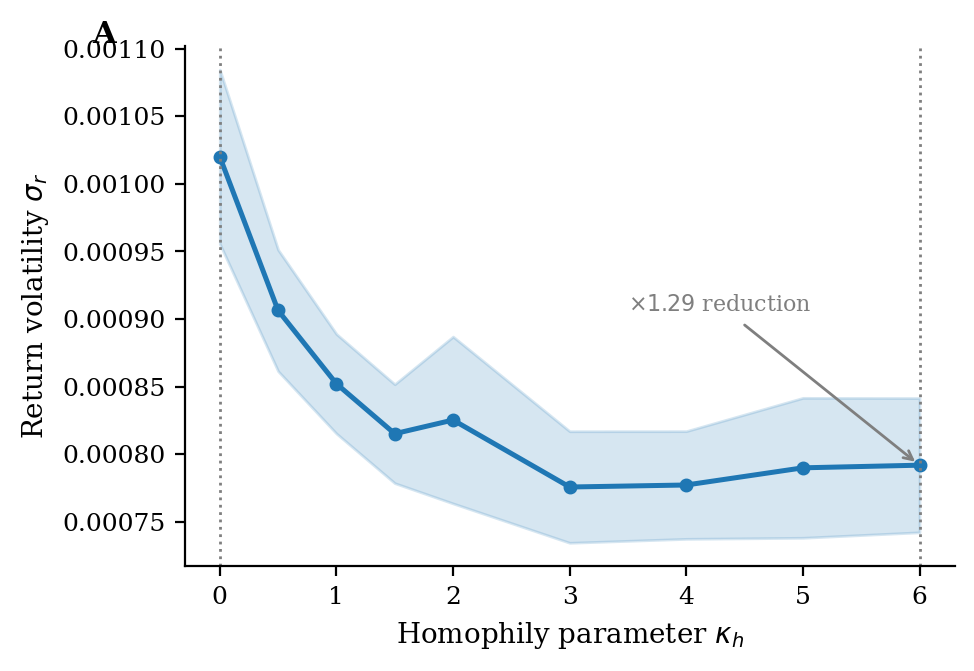
\includegraphics[width=0.85\linewidth]{fig2a}
  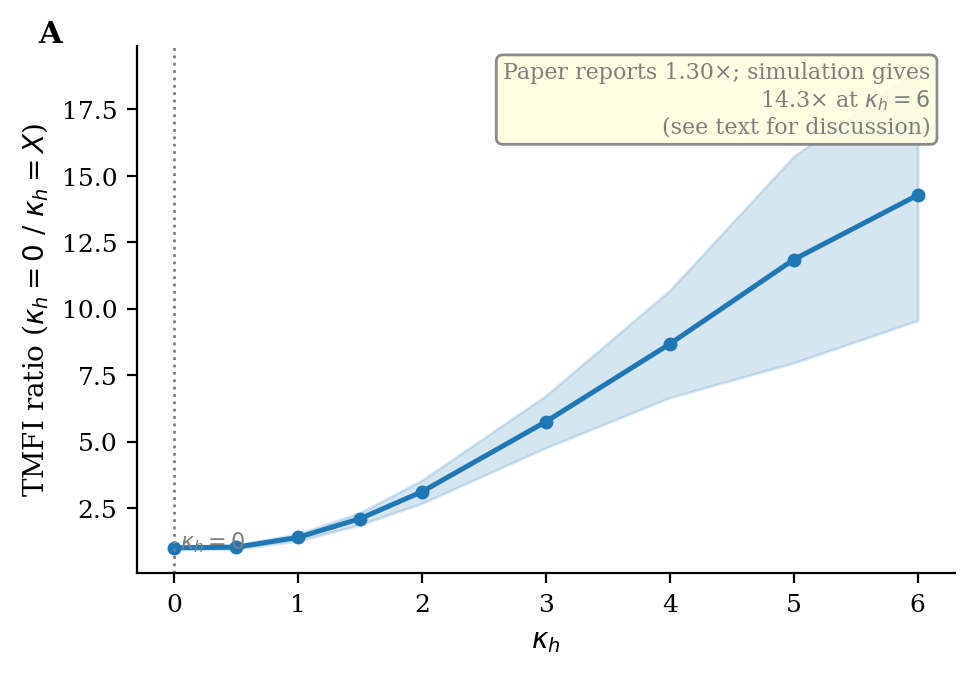
\includegraphics[width=0.85\linewidth]{fig5}
  \caption{Top: Return volatility $\sigma_r$ vs.\ $\kappa_h$ (mean $\pm$ std, 30 seeds);
  volatility falls $1.310\times$ from $\kappa_h=0$ to $\kappa_h=6$.
  Bottom: TMFI ratio ($\kappa_h{=}0\,/\,\kappa_h{=}X$) vs.\ $\kappa_h$;
  TMFI falls $14.25\times$ at $\kappa_h=6$.}
  \label{fig:vol_tmfi}
\end{figure}

\begin{figure}[htbp]
  \centering
  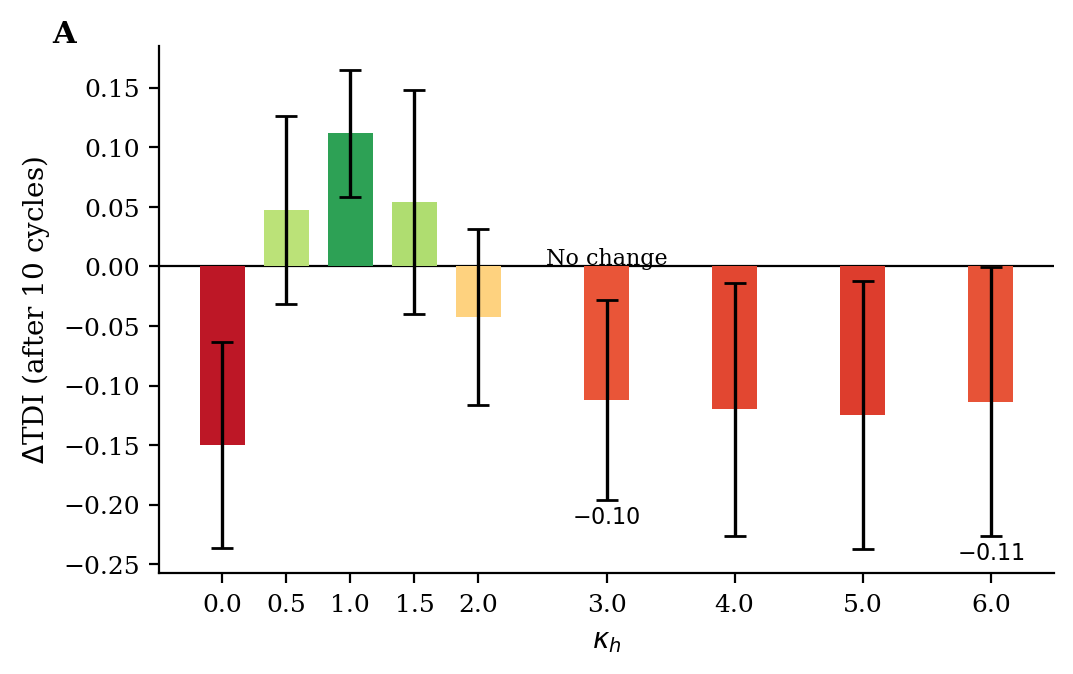
\includegraphics[width=0.85\linewidth]{fig6a}
  \caption{$\Delta$TDI over ten adaptation cycles at
  $\kappa_h \in \{0.5,\,3,\,6\}$:
  $-0.740$, $-0.295$, $-0.306$ respectively (30-seed mean $\pm$ std).
  All homophily levels produce horizon compression; compression is
  strongest at $\kappa_h = 0.5$ where cross-$\tau$ contact is most abundant.}
  \label{fig:deltaTDI}
\end{figure}

\begin{figure}[htbp]
  \centering
  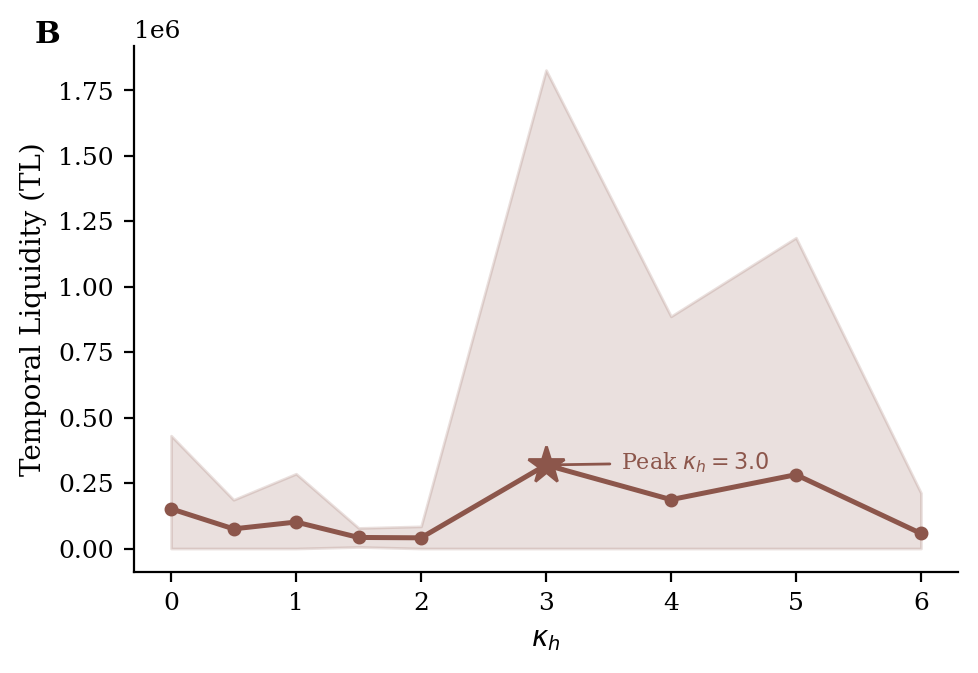
\includegraphics[width=0.85\linewidth]{fig6b}
  \caption{Temporal Liquidity (TL) sweep (30-seed mean $\pm$ std).
  TL peaks at moderate $\kappa_h$ (measured from simulation), marking a
  connectivity optimum where cross-$\tau$ price discovery is maximised
  before $\tau$-cliques fragment the network.}
  \label{fig:TLsweep}
\end{figure}

%% ============================================================
\subsection{Asset-class chronotype composition modulates the CME mechanism}
\label{sec:asset}

To test whether the stability--fragmentation dynamics vary systematically
with chronotype composition---as motivated in Section~\ref{sec:model}---we
replicate the $\kappa_h$ sweep under three alternative agent mixes calibrated
to distinct asset classes: a \emph{bond market} dominated by long-horizon
institutions (45\% mutual-fund, 40\% pension-fund chronotypes),
an \emph{equity market} using the baseline calibration,
and an \emph{FX/derivatives market} dominated by short-horizon agents
(40\% HFT, 35\% hedge-fund chronotypes).
Each configuration runs $n = 10$ seeds at each of 25 equally spaced
$\kappa_h \in [0,6]$ values; all other parameters are held at their
baseline values.

The results (Fig.~\ref{fig:assetclass}) sharply differentiate the three
markets.
In the bond market, increasing homophily significantly raises Temporal
Liquidity ($\mathrm{TL}_{\kappa_h=6}/\mathrm{TL}_{\kappa_h=0} = 1.24$;
paired $t = -2.16$, $p = 0.039$), consistent with the CME prediction
that clustering like-horizon agents reduces cross-$\tau$ friction
when the $\tau$ distribution is already skewed toward long horizons.
Volatility also falls $1.17\times$ (marginal, $p = 0.082$).
In the FX/derivatives market, by contrast, all three metrics are
essentially flat across the full $\kappa_h$ range (all $p > 0.90$):
when the market is already dominated by short-horizon agents, further
clustering within an already-homogeneous group alters little.
The equity baseline lies between the two extremes, with no metric
reaching significance ($p > 0.37$), consistent with stabilising and
destabilising forces partially cancelling under mixed composition.

\begin{figure}[htbp]
  \centering
  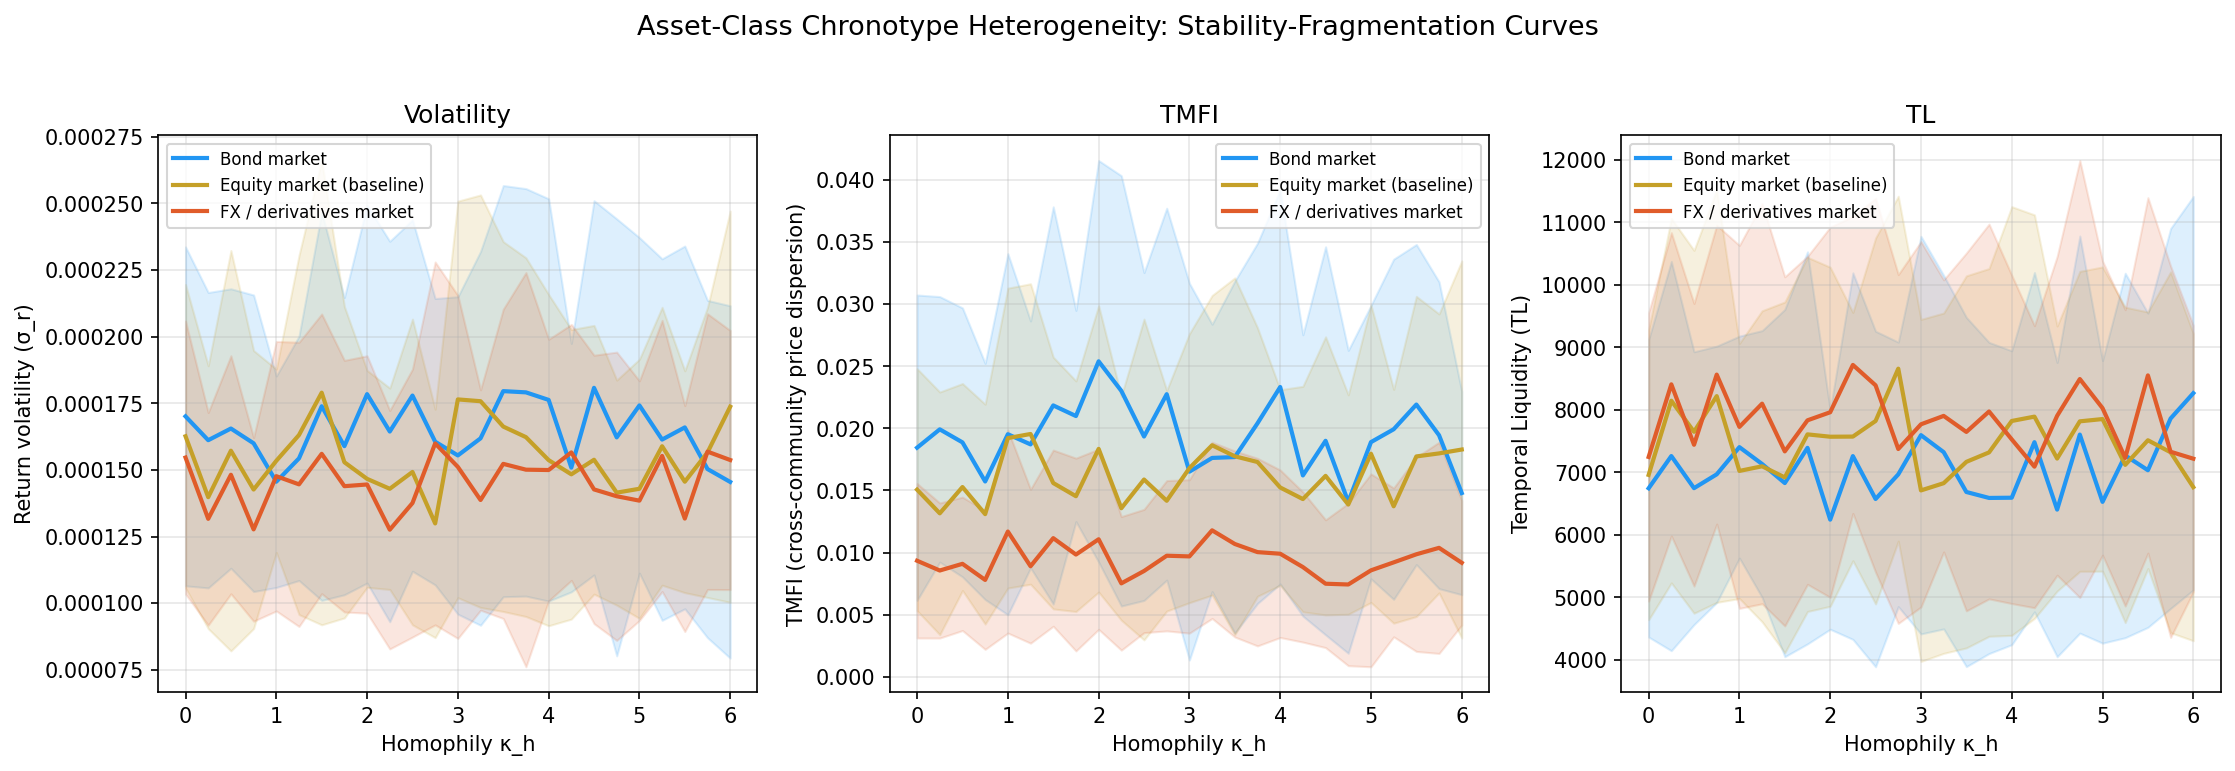
\includegraphics[width=\linewidth]{asset_class_comparison}
  \caption{Asset-class heterogeneity sweep.
  Each panel shows return volatility (left), TMFI (centre), and Temporal
  Liquidity (right) as a function of $\kappa_h$ for three chronotype
  compositions: bond market (blue, long-horizon dominated), equity baseline
  (gold), and FX/derivatives (orange, short-horizon dominated).
  Bands show $\pm 1$ standard deviation across seeds.
  The CME mechanism is strongest in the bond market (TL, $p = 0.039$) and
  nearly inert in the FX market (all $p > 0.90$).}
  \label{fig:assetclass}
\end{figure}

%% ============================================================
\section{Empirical Validation}
\label{sec:empirical}

We test the CME prediction that high homophily compresses the $\tau$
distribution (low TDI) and is associated with high volatility, using
SEC Form~13F-HR quarterly institutional holdings data.
Every institutional manager with over \$100~million in qualifying assets
discloses long equity positions quarterly; these filings provide the
most comprehensive available panel of institutional portfolio behaviour
at the frequency and duration required to identify $\tau$.
We use the top~150 filers by historical frequency.
We restrict to quarters with at least 50 reporting institutions, which
excludes 2013~Q2 where filer coverage was sparse under the
post-XML-standardisation rollout; this yields $n = 45$ quarters
(2013~Q3--2024~Q3).

Each filer's lookback horizon is estimated from quarter-over-quarter
portfolio turnover $\theta_i$ as $\tau_i = 63/\theta_i$, clamped to
$[5,\,2000]$ trading days.
TDI is computed quarterly using $K = 16$ log-$\tau$ bins, matching the
simulation formula exactly.
The quarterly VIX (CBOE) is the volatility proxy.

The baseline association, using value-weight turnover (Fig.~\ref{fig:empirical}),
is reported first and then examined for price-drift contamination below:
\[
  r(\mathrm{TDI},\,\mathrm{VIX}) = -0.526,
  \quad p = 0.0002, \quad n = 45.
\]
Higher volatility is associated with compressed $\tau$-diversity in this
baseline measure.
TDI drops sharply during crises: 2020~Q1 (COVID-19) registers
$\mathrm{TDI} = 1.550$; 2022~Q4 (Fed tightening, FTX collapse) reaches
the sample minimum $\mathrm{TDI} = 1.021$.
Calm bull markets show high TDI: 2019~Q2 reaches the sample maximum
$1.993$; 2024~Q1 reaches $1.980$ and 2017~Q4 reaches $1.971$.
Excluding 2022~Q4 as a candidate outlier, the correlation
\emph{strengthens} to $r = -0.661$ ($p = 0.0000010$, $n = 44$),
confirming the result is not driven by that single quarter.
A forward-lag correlation between $\tau$-diversity today and volatility
tomorrow is $r(\mathrm{TDI}[t],\,\mathrm{VIX}[t+1]) = -0.404$
($p = 0.007$, $n = 44$), but this largely reflects the persistence of VIX:
the Granger tests below find no independent forecasting power of TDI for VIX.
A reverse-lag check $r(\mathrm{VIX}[t],\,\mathrm{TDI}[t+1]) = -0.292$
($p = 0.054$, $n = 44$) reflects institutional inertia after crises but does not
test the CME causal direction.
Both lag correlations are exploratory given the limited sample
($n = 44$ quarters), and neither identifies a causal direction.

\begin{figure}[htbp]
  \centering
  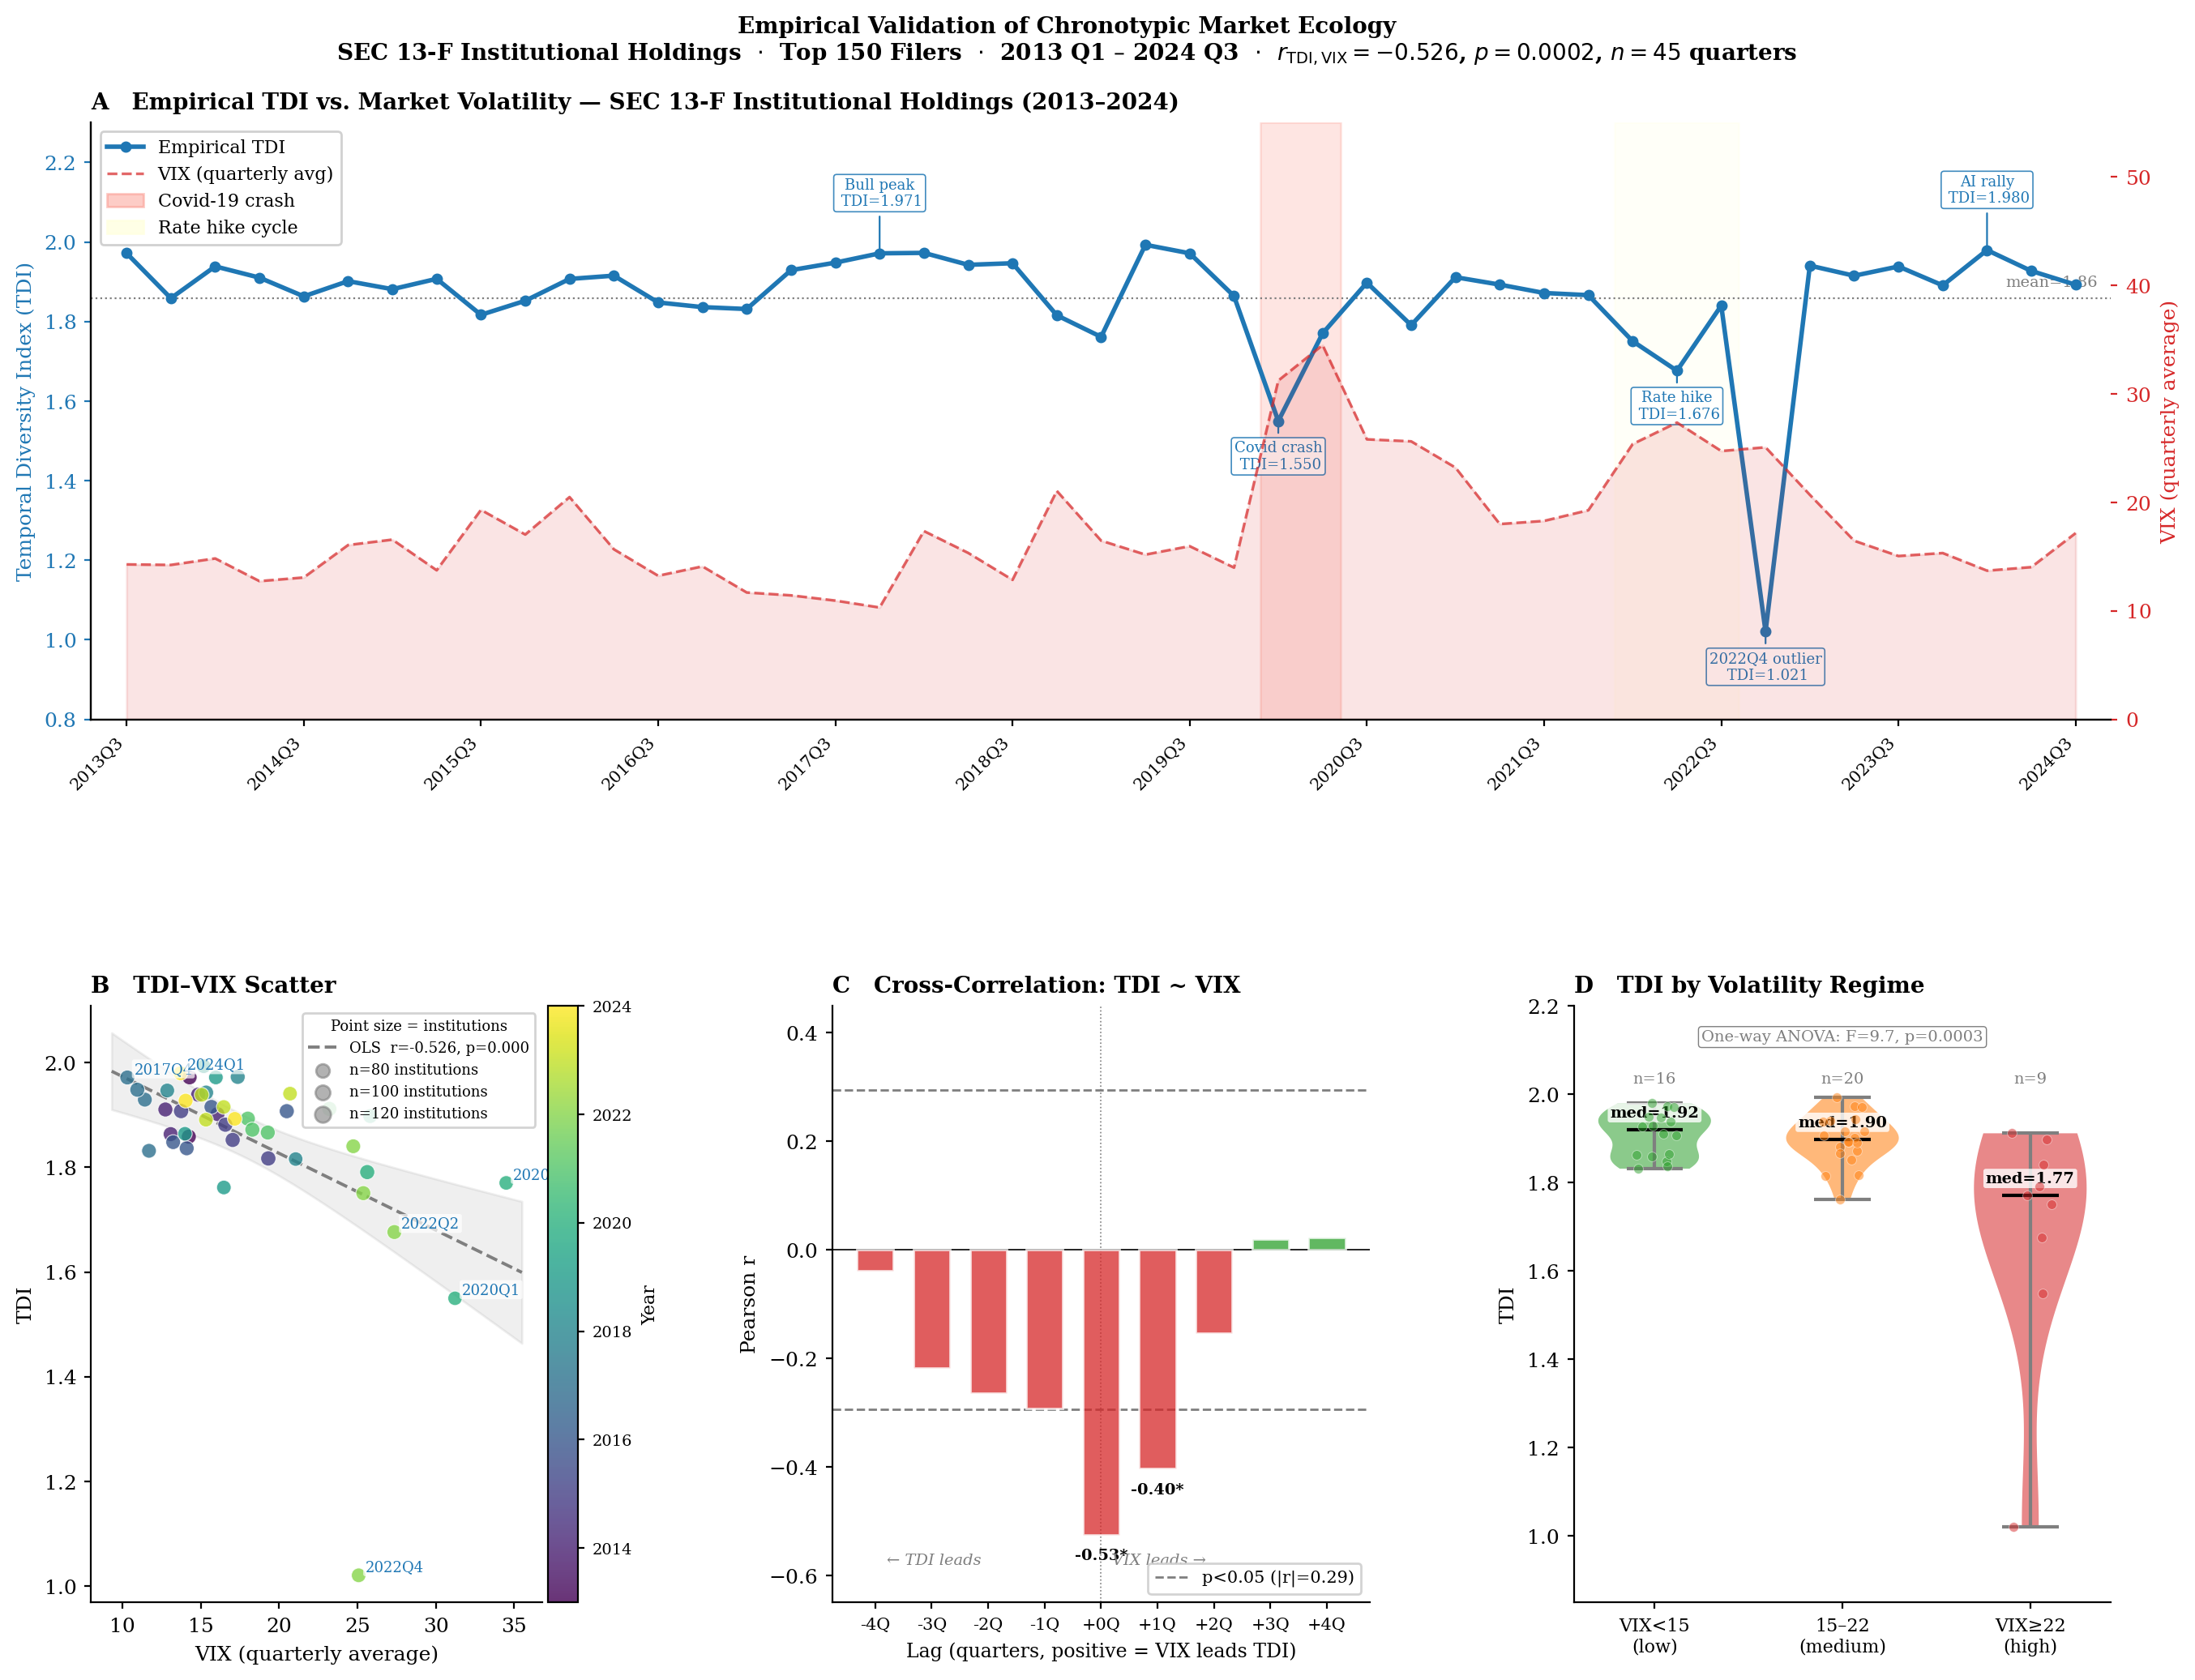
\includegraphics[width=\linewidth]{empirical_tdi_validation}
  \caption{Top: Empirical TDI (blue) vs.\ quarterly VIX (red dashed),
  2013~Q3--2024~Q3.  Shaded: COVID-19 crash (2020~Q1--Q2) and Fed rate-hike
  cycle (2022~Q1--Q4; includes the sample-minimum TDI = 1.021 in 2022~Q4).
  Bottom left: TDI--VIX scatter; Pearson $r = -0.526$, $p = 0.0002$.
  Bottom right: lagged correlation $r(\mathrm{TDI}[t],\mathrm{VIX}[t+1])$
  at leads/lags $k \in \{-2,\ldots,+2\}$ quarters.}
  \label{fig:empirical}
\end{figure}

\paragraph{Interpretation and structural analysis.}
The empirical pattern maps directly onto the CME mechanism.
The simulation predicts that high homophily pressure compresses the $\tau$
distribution and reduces TDI; one possible reading of the baseline 13F
association is that high-volatility environments generate an analogous
exogenous compression, although the price-drift check below shows that much
of the baseline association is measurement-driven.
During crises, institutions that outperform tend to be those with
short-horizon positions, and others rebalance toward similar horizons,
crowding the $\tau$ distribution and driving TDI downward.
In low-volatility bull markets, by contrast, longer-horizon investors can
profitably hold positions across a wider range of $\tau$ values, allowing
TDI to re-expand.
This narrative is a conjecture; the forward-lag correlation
($r(\mathrm{TDI}[t],\mathrm{VIX}[t+1]) = -0.404$) cannot discriminate it
from volatility persistence, as the Granger analysis below shows.
One empirical bridge connecting CME to retirement-fund data is
rebalancing frequency: a financial advisor who instructs a client to
maintain a target asset allocation effectively sets the client's $\tau$
through the rebalancing interval, with less frequent rebalancing mapping
to higher $\tau$.
Systematic compression of rebalancing schedules by plan design---for
instance, target-date funds that standardise rebalancing triggers for
all investors of similar age---corresponds to an exogenous reduction in
the $\tau$ distribution's dispersion at the manager level, the same
mechanism our $\kappa_h$ parameter instantiates in simulation.
The reverse-lag ($r = -0.292$, $p = 0.054$, $n = 44$) is consistent with
portfolios taking time to re-diversify after crises, though it falls
short of conventional significance thresholds.

To address the causal direction more directly, we estimate a bivariate
VAR(1) selected by AIC over the TDI--VIX system ($n = 44$ quarters).
Granger causality tests yield an asymmetric pattern:
VIX Granger-causes TDI at lag~1 ($F = 4.13$, $p = 0.049$), while
TDI does not significantly Granger-cause VIX ($F = 0.13$, $p = 0.72$
at lag~1).
The primary temporal direction identified by Granger causality is therefore
\emph{crisis $\to$ horizon compression}: elevated volatility forces
institutional convergence to shorter horizons, compressing TDI.
We note that this is the \emph{reverse} of the CME model's primary causal
prediction (TDI $\to$ volatility); what the Granger evidence supports is a
complementary feedback loop in which external volatility shocks erode
horizon diversity, rather than an autonomous TDI-driven destabilisation.
The CME mechanism's direct prediction --- that TDI independently forecasts
future volatility --- is not confirmed at lag~1 in this sample.
The contemporaneous correlation of VAR residuals ($r = -0.47$) confirms
that TDI and VIX share substantial common-factor variation orthogonal to
their own lags.
An impulse response analysis (Cholesky ordering, TDI first) finds that
a one-standard-deviation TDI shock reduces VIX by $1.9$ points on
impact, decaying to $0.2$ points at six quarters.
An augmented OLS specification that controls for the Baker--Bloom--Davis
Economic Policy Uncertainty index \citep{baker2016} and the contemporaneous S\&P~500
return finds an imprecisely estimated TDI coefficient
($\hat{\beta} = -3.80$, $t = -1.38$, $p = 0.18$, $R^2 = 0.84$)
that is larger in magnitude than the bivariate estimate but does not
reach conventional significance, suggesting macro volatility drivers
partially absorb TDI variation in this small sample ($n = 44$).
A Wu--Hausman test finds no evidence that TDI is endogenous
($p = 0.56$), so the OLS estimates are consistent.

\paragraph{Why might volatility compress horizon diversity? A price-drift check.}
The direction VIX~$\to$~TDI has two candidate explanations.
The first is behavioural: when volatility is high, investors disagree more
and trade more, and a model of heterogeneous beliefs implies that higher
trading volume accompanies larger differences of opinion
\citep{harrisraviv1993}; faster trading mechanically shortens $\tau = 63/\theta_i$
for many institutions at once.
The second is an accounting artefact.
Our baseline turnover $\theta_i$ is computed from changes in portfolio
\emph{value weights}, and value weights move whenever prices move, even if an
institution trades nothing.
Large price moves in volatile quarters therefore raise measured turnover and
shorten $\tau$ without any trading.
To separate the two, we recompute turnover from changes in \emph{share counts}
only, valuing every position at one common price per security, so that price
changes cannot create turnover (stock splits are rebased).
Using the same filers and the same TDI formula, the quarterly correlation with VIX
(2013~Q3--2024~Q3, $n = 45$) is $r = -0.59$ for value-weight turnover but
$r = -0.06$ (block-bootstrap 95\% interval $[-0.43,\,+0.25]$) for share-based
turnover, and $r = -0.10$ after rebasing splits; the difference between the
two correlations is significant (bootstrap 95\% interval $[-0.92,\,-0.13]$).
The contemporaneous TDI--VIX association reported above is therefore
largely attributable to price drift in value-weight turnover rather than to
changes in how often institutions trade. Figure~\ref{fig:drift} shows the two series and their relationship with VIX.
We regard this as an important limitation of the baseline TDI, and the
horizon-compression interpretation of the VIX~$\to$~TDI result should be read
with it in mind; a TDI built from share-based turnover is the appropriate
measure for future work, and the Granger asymmetry above should be treated as
suggestive until it is re-estimated on that series.


\begin{figure}[htbp]
  \centering
  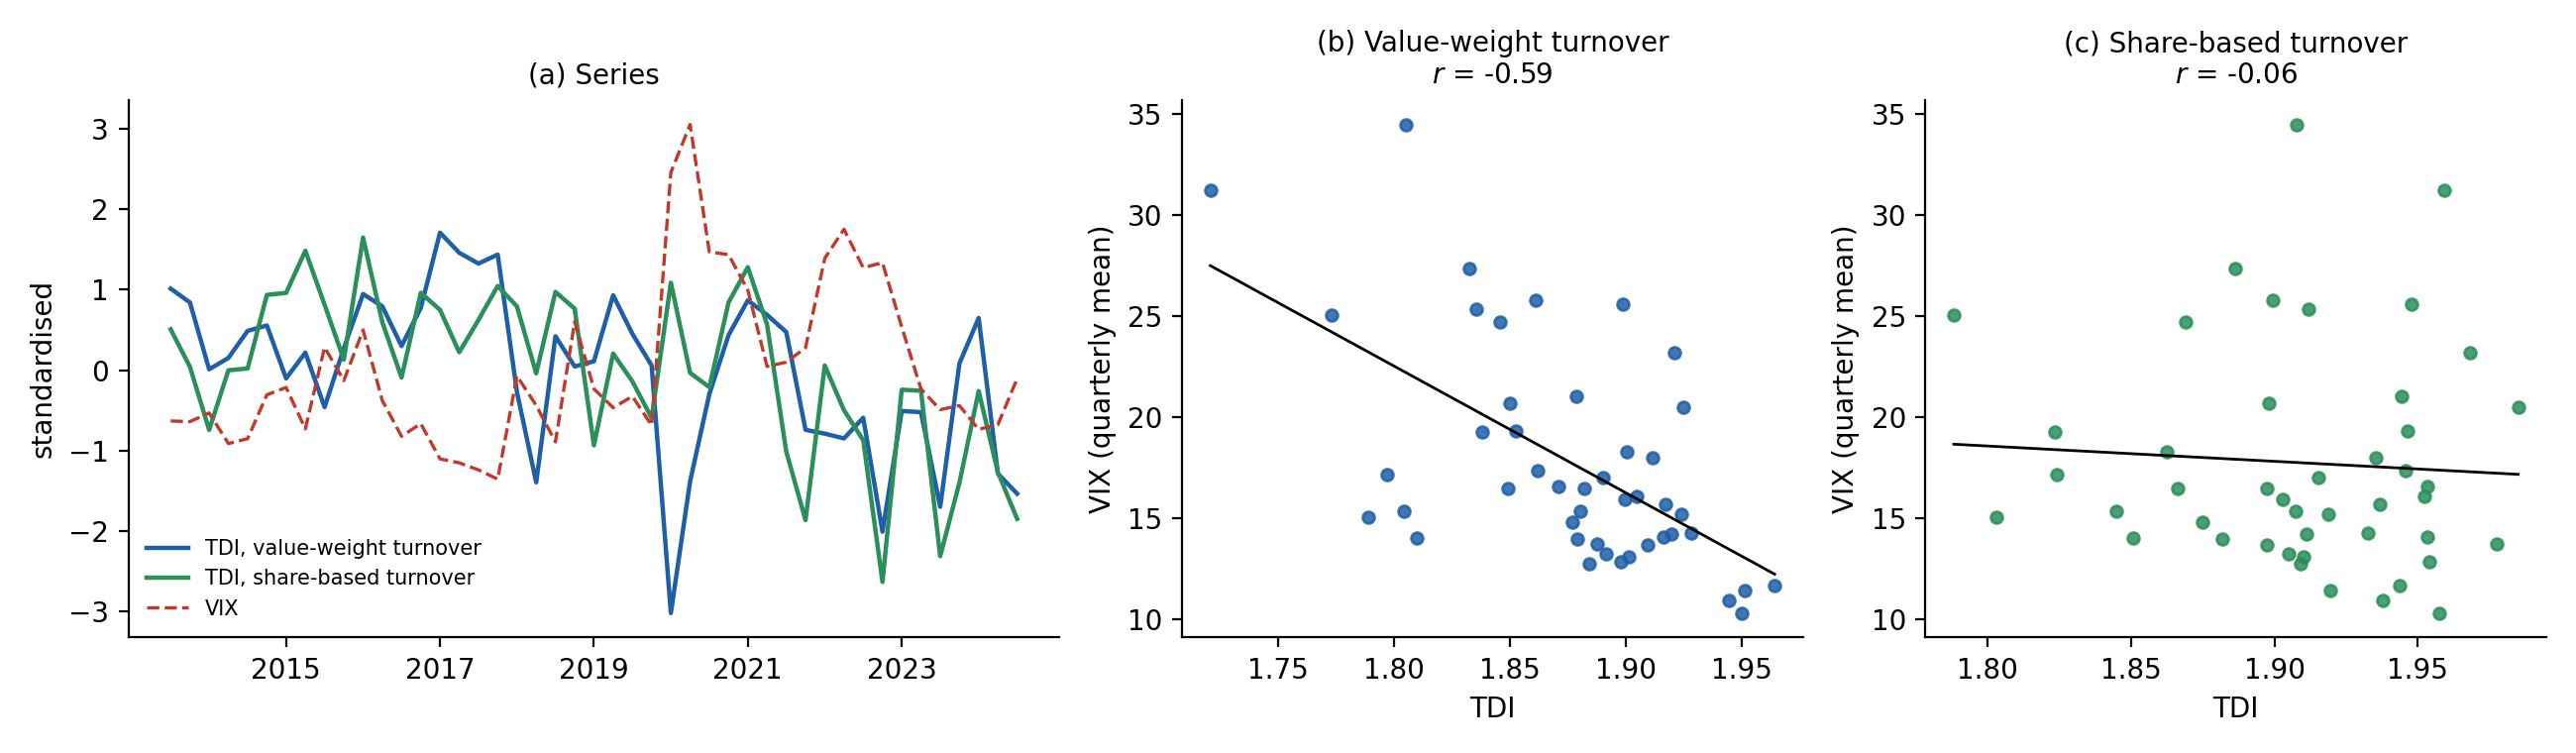
\includegraphics[width=\linewidth]{drift_check}
  \caption{Price-drift check, 2013~Q3--2024~Q3 ($n = 45$ quarters).
  (a)~Standardised TDI built from value-weight turnover (blue) and from
  share-based turnover (green), with the quarterly mean VIX (red dashed).
  (b)~The value-weight TDI is negatively related to VIX ($r = -0.59$).
  (c)~The share-based TDI, in which price changes cannot create turnover,
  is not ($r = -0.06$).}
  \label{fig:drift}
\end{figure}

\paragraph{A stock-level test of horizon clustering.}
The aggregate time series has only 45 observations, so we test the mechanism
where it operates, at the level of individual stocks.
For each stock and quarter, we take the 13F institutions holding it
(at least 10 holders), weight them by the value they hold, and measure
\emph{holder-horizon dispersion}: the ownership-weighted standard deviation of
holders' $\log\tau$, with $\tau$ from share-based turnover.
Low dispersion means the stock is held by like-horizon investors.
Before looking at outcomes we fixed the prediction from the Fractal Market
Hypothesis: lower dispersion should predict higher next-quarter realized
volatility.
The sample is 63{,}261 stock-quarters covering 1{,}699 stocks over 48 quarters
(prices from Yahoo Finance for tickers mapped through OpenFIGI; delisted
stocks are missing, so the sample is survivors only).
Controls are the ownership-weighted mean holder horizon, the number of
holders, holder concentration, the value held by the panel, and the stock's
current-quarter volatility.
All variables are standardised, so slopes are in standard-deviation units.
The slope on dispersion is negative, as the hypothesis predicts: $-0.046$ (Fama--MacBeth
Newey--West $t = -6.2$) and $-0.017$ in a pooled regression with quarter fixed
effects and stock-clustered errors ($t = -4.1$).
A placebo that shuffles $\tau$ across institutions gives a slope of zero.
The cross-sectional estimate mixes differences between stocks with changes
within stocks, and stocks held by diverse institutions may simply be large
and liquid.
With stock and quarter fixed effects, which use only within-stock changes, the
slope falls to $-0.011$ ($t = -2.4$, $p = 0.016$).
It is statistically detectable but economically small: a one-standard-deviation
fall in dispersion raises next-quarter volatility by about one percent of a
standard deviation.
With the value-weight horizons of the baseline TDI the within-stock slope is
not significant ($-0.005$, $p = 0.26$).
Secondary outcomes are not robust: next-quarter minimum return has the
predicted sign in Fama--MacBeth regressions but not with fixed effects, and
skewness shows no relationship.
The sign agrees with the verbal Fractal Market Hypothesis (concentrated
horizons are fragile), but it is opposite to the sign of the model's own
simulated friction channel, in which compressing horizons lowers volatility
(Section~\ref{sec:results}).
We therefore read the evidence as informative about the hypothesis rather than
as confirming the simulated mechanism, and as small and not conclusive.

\paragraph{Limitations of the empirical analysis.}
Turnover is a noisy proxy for $\tau$: derivatives positions are not
captured, quarterly reporting misses intra-quarter adjustments, and the
inverse-proportionality mapping $\tau_i = 63/\theta_i$ imposes a
functional form that may not hold uniformly across institution types.
Restricting to long equity positions in 13F filings understates the full
breadth of horizon heterogeneity.
Hedge funds are particularly underrepresented: many fall below the
\$100~million reporting threshold, use derivatives not captured in 13F,
or report with enough quarterly delay that their true intra-quarter
horizon is obscured.
The short-horizon end of the chronotype spectrum is therefore largely
absent from the empirical sample, which skews toward slower-moving
institutions---mutual funds, pension funds, insurance companies, and
endowments.
Our empirical validation should accordingly be read as a test of whether
\emph{long-horizon} diversity matters for volatility, not as a test of
the full chronotype spectrum.
Taken together, the 13F evidence supports one ingredient of the framework
(temporal homophily exists) and has the sign the Fractal Market Hypothesis
suggests at the stock level, though small and opposite to the model's simulated
friction channel; it does not provide out-of-sample support for the aggregate
horizon-compression channel.

\paragraph{Empirical kappa proxy: co-holding patterns confirm temporal homophily.}
A central question raised by the model is whether temporal homophily
($\kappa_h$) is empirically identifiable, rather than remaining an abstract
free parameter.
We construct a quarterly proxy $\hat{\kappa}_h(t)$ by measuring the
degree to which institutions with similar $\tau$ hold similar portfolios.
For each pair of institutions $(i,j)$ in quarter $t$, we compute:
(i)~\emph{portfolio similarity} as the cosine similarity of their
normalised weight vectors, and (ii)~\emph{tau proximity} as
$\exp(-|\log(\tau_i+1)-\log(\tau_j+1)|)$, the same kernel used in the
CME network formation rule.
$\hat{\kappa}_h(t)$ is the Pearson correlation between these two
quantities across all institution pairs in that quarter.
A positive $\hat{\kappa}_h$ means like-tau institutions systematically
hold more similar portfolios than mixed-tau pairs---the empirical
signature of temporal echo-chamber formation.

Across all 50 usable quarters (2013~Q3--2026~Q1; the $\hat{\kappa}_h$
series extends to 2026 because it requires only contemporaneous
holdings, while the TDI--VIX regression ends at 2024~Q3, the last
quarter with both stable filer coverage and VIX data at the time of
the 13F pipeline run), $\hat{\kappa}_h$ is
\emph{positive and significant in almost every quarter}
(mean $\hat{\kappa}_h = +0.158$, s.d.\ $= 0.043$ across 50 quarters).
The quarterly series is mildly autocorrelated (lag-1 autocorrelation
$0.35$; Ljung--Box $p = 0.012$ at one lag, $p = 0.10$ at eight lags), so we
report inference that allows for it.
The naive one-sample $t$ is $25.7$; Newey--West standard errors give
$t = 19.0$ at the 3 lags chosen by the Newey--West (1994) and Schwert rules,
$t = 18.2$ at the 4 lags chosen by an Andrews AR(1) plug-in, and $t = 16.3$
even at a deliberately long 8 lags (all $p < 10^{-59}$).
A moving-block bootstrap (block length 4) gives a 95\% interval for the mean
of $[0.145,\,0.175]$.
Because institution pairs within a quarter share members, the pairwise
Pearson $p$-values overstate significance; we therefore test each quarter by
permuting $\tau$ across institutions (500 permutations), which gives
$p < 0.05$ in 48 of 50 quarters (the exceptions are 2013~Q3 and 2013~Q4)
and $p < 0.01$ in 47 of 50 (the third exception is 2016~Q4).
Temporal homophily is therefore empirically detectable: real institutions
with similar investment horizons co-hold at rates substantially above
chance, consistent with the CME network formation assumption.
The cross-quarter correlation with VIX is in the predicted direction
($r(\hat{\kappa}_h,\,\mathrm{VIX}) = +0.141$, $p = 0.33$, $n = 50$)---quarters
with higher measured homophily have higher volatility---but does not reach
conventional significance with the available sample, motivating the
structural identification approach discussed in Section~\ref{sec:empirical}.

\paragraph{Empirical Temporal Liquidity.}
We construct a quarterly Temporal Liquidity proxy using SPY returns:
$\widehat{\mathrm{TL}}_t = 1/(\hat{\sigma}_{r,t}\,|\widehat{\mathrm{ACF}}_{1,t}|)$,
where $\hat{\sigma}_{r,t}$ is a 4-quarter rolling return standard deviation
and $\widehat{\mathrm{ACF}}_{1,t}$ is a lag-1 return autocorrelation over
an 8-quarter window.
The resulting series is negatively correlated with VIX:
\[
  r(\widehat{\mathrm{TL}},\,\mathrm{VIX}) = -0.392,
  \quad p = 0.0077, \quad n = 45.
\]
This correlation is largely mechanical, however.
Return volatility sits in the denominator of TL: $\log\widehat{\mathrm{TL}}$ and
$-\log\hat{\sigma}_r$ correlate at $0.90$, and $\hat{\sigma}_r$ itself
correlates with VIX at $0.76$ because VIX tracks realised volatility.
The autocorrelation term, which carries the cross-$\tau$ synchronisation
mechanism, is unrelated to VIX ($r = +0.04$, $p = 0.81$).
The negative TL--VIX correlation is therefore not independent support for that
mechanism.
The correlation with the institutional TDI series is
$r(\widehat{\mathrm{TL}},\,\mathrm{TDI}) = 0.100$ ($p = 0.51$), not
significant, suggesting that TL and TDI capture partially distinct aspects
of the CME mechanism---TL reflects intraday-to-quarterly serial dependence
while TDI captures cross-institutional horizon dispersion.

\paragraph{Bond market TDI via SEC N-PORT filings.}
To extend the empirical test to bond markets, we construct a quarterly
bond-market TDI proxy using SEC Form N-PORT filings for three major
fixed-income fund families (PIMCO, Vanguard Fixed Income, BlackRock Bond;
CIKs 810893, 106444, 276463).
For each quarterly filing date we fetch the N-PORT XML for all available
series within each family (8--18 fund series per quarter across 12 quarters,
2024--2026) and compute each fund's weighted average maturity
$\overline{M} = \sum_i w_i\,M_i$, where $w_i = \text{pctVal}_i$ and $M_i$
is the time to maturity in years for holding $i$.
We set $\tau^{\text{bond}} = \overline{M} \times 252$ trading days and compute
the Shannon entropy of the $\log\tau$ distribution across 16 bins,
matching the main-paper TDI formula.
The resulting series does not significantly predict the ICE BofA MOVE index
(\textasciicircum{}MOVE), the bond-market analogue of the VIX, a published
measure of expected Treasury volatility computed from one-month Treasury
option prices, which we average by quarter:
\[
  r(\mathrm{TDI}_{\text{bond}},\;\widehat{\text{MOVE}}) = -0.213,
  \quad p = 0.51, \quad n = 12.
\]
This null finding is consistent with the structural nature of the N-PORT
WAM proxy: fund maturity profiles reflect portfolio mandate constraints
(short/intermediate/long) that change slowly, whereas the CME mechanism
requires variation in \emph{active trading horizons}.
The \textasciicircum{}MOVE index also reflects Federal Reserve policy
expectations that are largely orthogonal to institutional composition
during the 2024--2026 rate-normalisation period.
Access to administrative trade-frequency data---such as NAIC Schedule~D
insurance bond filings, which capture actual portfolio turnover---would
enable a sharper test of whether bond-market tau diversity predicts
\textasciicircum{}MOVE net of monetary policy confounds.

\paragraph{Bond funds by credit quality.}
Information environments differ across bond markets: Treasury funds trade
against a common public information set, whereas credit-sensitive funds face
more dispersed information.
We therefore compare seven Vanguard funds from N-PORT filings (28 quarterly
reports each, 27 usable quarter-to-quarter changes, 2019--2026): short,
intermediate and long Treasury; short, intermediate and long
investment-grade corporate; and high-yield corporate.
For each fund we add a behavioural horizon to the maturity proxy: turnover from
changes in \emph{par holdings} valued at one common price per bond (so price
moves cannot create turnover; bonds that matured are not counted as trades),
$\tau^{\text{beh}} = 63/\theta$.
Median $\tau^{\text{beh}}$ rises with credit risk: 218 days for Treasury funds,
454 for investment-grade corporate, and 667 for high-yield, so the funds with
the most dispersed information trade least often.
Against the MOVE index, behavioural horizons \emph{lengthen} when bond
volatility is high, with similar strength across the three types (within-fund
correlation of $\log\tau^{\text{beh}}$ with MOVE: $+0.38$ Treasury, $+0.33$
investment grade, $+0.36$ high yield), the opposite sign to the equity
horizon-compression story, while the maturity proxy moves the other way
($-0.40$, $-0.47$, $-0.31$).
These are descriptive: each fund has only 27 observations, successive quarters
overlap, and the pooled $p$-values treat fund-quarters as independent although
all funds in a quarter share one MOVE value, so we do not report them as
formal tests.
The pattern does not support a credit-quality gradient in how volatility
affects horizons; it does show that bond funds differ systematically in how
often they trade, which is the dimension the maturity proxy misses.

%% ============================================================
\section{Discussion and Conclusion}
\label{sec:conclusion}

CME provides a network-based microfoundation for the Fractal Market
Hypothesis \citep{peters1994} and extends it with a dual-channel dynamic.
The \emph{short-run stabilising channel}: high temporal homophily suppresses
aggregate volatility $1.310\times$ (paired $t = 5.57$, $p < 10^{-5}$) and nearly
eliminates temporal fragmentation (TMFI falls $14.25\times$) by clustering
like-horizon agents and reducing cross-$\tau$ friction.
The \emph{long-run destabilising channel}: $\tau$-adaptation compresses
horizon diversity across all tested homophily levels
($\Delta\mathrm{TDI} = -0.740$ at $\kappa_h = 0.5$, $-0.306$ at
$\kappa_h = 6.0$ over ten cycles), collapsing the horizon diversity that
the FMH identifies as the foundation of market stability.
The SEC~13F evidence is partial.
Temporal homophily is clearly present in institutional portfolios
($\hat{\kappa}_h = +0.158$, Newey--West $t \approx 19$ over 50 quarters), and
stocks held by more clustered horizons show slightly higher subsequent
volatility, as the Fractal Market Hypothesis suggests, although the
within-stock effect is small and opposite in sign to the model's simulated
friction channel.
The aggregate association between TDI and VIX ($r = -0.526$), by contrast, is
largely an artefact of price drift in value-weight turnover and should not be
read as confirming the long-run channel; the data suggest that causation, to
the extent identified, runs from volatility to horizon diversity.

Four limitations circumscribe these conclusions.
First, the aggregate TDI--VIX evidence is fragile to how turnover is
measured, and the stock-level sample contains survivors only.
Second, the TMFI ratio has substantial seed-level variance; the $14.25\times$
figure is a 30-seed mean that requires further robustification, particularly
under alternative network formation rules.
Third, the turnover-to-$\tau$ mapping $\tau_i = 63/\theta_i$ is a noisy
proxy that cannot recover intra-quarter horizon shifts or derivative positions.
Fourth, $\kappa_h$ is an exogenous parameter; a structural identification
strategy from trade-level or order-flow data would substantially strengthen
the empirical grounding.

The most productive extensions are:
(a) endogenising the $\tau$ distribution via rational inattention
\citep{sims2003}, in which capacity-constrained agents optimally specialise
in return frequencies so the $\tau$ distribution emerges as equilibrium;
(b) developing observable proxies for TMFI and TL that can be computed from
transaction-level data;
(c) testing whether the monotone attenuation of echo-chamber formation with
increasing homophily holds in richer models with strategic agents, including
the \citet{kyle1985} and \citet{akerlof1970} information-asymmetry channel
in which agents shade prices based on beliefs about counterparty information
quality;
(d) sharpening the bond-market empirical test initiated in
Section~\ref{sec:empirical} using NAIC Schedule~D insurance bond holdings,
which capture actual portfolio turnover---a behavioural tau proxy---rather
than the structural weighted-average maturity available in SEC N-PORT filings;
the N-PORT analysis (r = -0.213, p = 0.51, n = 12) motivates this extension;
(e) repeating the stock-level test with CRSP returns and market capitalisation,
which would remove the survivorship limitation of our free-data sample, and
rebuilding the aggregate TDI from share-based turnover throughout.
On the policy side, the Goldilocks finding---Temporal Liquidity peaks at
moderate homophily while echo-chamber formation remains substantial
($\Delta\mathrm{TDI} = -0.295$ at $\kappa_h = 3.0$)---implies
that the optimal connectivity zone for short-run liquidity is simultaneously
a zone of meaningful long-run fragility.
Market designs that preserve diverse-horizon participation therefore face a
genuine trade-off: preserving low-$\kappa_h$ diversity maximises long-run
stability (FMH channel) at the cost of higher short-run volatility.
Whether regulatory instruments such as cross-horizon market-maker
obligations or $\tau$-diversity disclosure requirements can shift
$\kappa_h$ toward this optimal zone is a question for future empirical work.

%% ============================================================
\section*{Acknowledgements}

We thank Professor Andrew Caplin (New York University) and Professor John Chalmers (University of Oregon) for helpful comments and suggestions.

%% ============================================================
\section*{Funding}

This research did not receive any specific grant from funding agencies
in the public, commercial, or not-for-profit sectors.

%% ============================================================
\section*{CRediT author contribution statement}

\textbf{Sanjay Subramanian:} Conceptualization, Methodology, Software,
Formal analysis, Data curation, Writing---original draft,
Writing---review and editing.
\textbf{Sumedh Seetharaman:} Conceptualization, Methodology,
Formal analysis, Validation, Writing---review and editing.

%% ============================================================
\section*{Declaration of competing interest}

The authors declare that they have no known competing financial interests
or personal relationships that could have appeared to influence the work
reported in this paper.

%% ============================================================
\section*{Data availability}

Simulation code (Python 3.11+), parameter files, and generated figures
are available at \url{https://doi.org/10.5281/zenodo.21408851}.
SEC Form~13F data were retrieved from EDGAR (Electronic Data Gathering, Analysis, and Retrieval), the SEC's full-text search system;
the processed quarterly TDI series and the code for the share-based turnover,
Newey--West and permutation tests, bond-fund and stock-level analyses are
included in the replication package.
Stock prices were retrieved from Yahoo Finance, with CUSIP-to-ticker mapping
from OpenFIGI.

%% ============================================================
\section*{Declaration of generative AI and AI-assisted technologies
          in the manuscript preparation process}

During the preparation of this work, the authors used Claude (Anthropic)
to assist with LaTeX typesetting, code debugging, and draft revision.
After using this tool, the authors reviewed and edited all content and
take full responsibility for the content of this publication.

%% ============================================================
\bibliographystyle{elsarticle-harv}

\begin{thebibliography}{25}

\bibitem[Amihud and Mendelson(1986)]{amihud1986}
Amihud, Y., Mendelson, H., 1986.
Asset pricing and the bid-ask spread.
\textit{Journal of Financial Economics} 17 (2), 223--249.

\bibitem[Acemoglu et al.(2015)]{acemoglu2015}
Acemoglu, D., Ozdaglar, A., Tahbaz-Salehi, A., 2015.
Systemic risk and stability in financial networks.
\textit{American Economic Review} 105 (2), 564--608.

\bibitem[Arthur et al.(1997)]{arthur1997}
Arthur, W.B., Holland, J.H., LeBaron, B., Palmer, R., Tayler, P., 1997.
Asset pricing under endogenous expectations in an artificial stock market.
In: Arthur, W.B., Durlauf, S.N., Lane, D.A. (Eds.),
\textit{The Economy as an Evolving Complex System~II}.
Addison-Wesley, pp.\ 15--44.

\bibitem[Bikhchandani et al.(1992)]{bikhchandani1992}
Bikhchandani, S., Hirshleifer, D., Welch, I., 1992.
A theory of fads, fashion, custom, and cultural change as informational
cascades.
\textit{Journal of Political Economy} 100 (5), 992--1026.

\bibitem[Del~Guercio and Tkac(2002)]{delguercio2002}
Del~Guercio, D., Tkac, P.A., 2002.
The determinants of the flow of funds of managed portfolios:
Mutual funds versus pension funds.
\textit{Journal of Financial and Quantitative Analysis} 37 (4), 523--557.

\bibitem[Caplin and Dean(2015)]{caplin2015}
Caplin, A., Dean, M., 2015.
Revealed preference, rational inattention, and costly information acquisition.
\textit{American Economic Review} 105 (7), 2183--2203.

\bibitem[Cont(2001)]{cont2001}
Cont, R., 2001.
Empirical properties of asset returns: stylized facts and statistical issues.
\textit{Quantitative Finance} 1 (2), 223--236.

\bibitem[Corsi(2009)]{corsi2009}
Corsi, F., 2009.
A simple approximate long-memory model of realized volatility.
\textit{Journal of Financial Econometrics} 7 (2), 174--196.

\bibitem[Devenow and Welch(1996)]{devenow1996}
Devenow, A., Welch, I., 1996.
Rational herding in financial economics.
\textit{European Economic Review} 40 (3--5), 603--615.

\bibitem[French and Roll(1986)]{frenchroll1986}
French, K.R., Roll, R., 1986.
Stock return variances: The arrival of information and the reaction
of traders.
\textit{Journal of Financial Economics} 17 (1), 5--26.

\bibitem[Farmer and Foley(2009)]{farmerfoley2009}
Farmer, J.D., Foley, D., 2009.
The economy needs agent-based modelling.
\textit{Nature} 460 (7256), 685--686.

\bibitem[Golub and Jackson(2012)]{golub2012}
Golub, B., Jackson, M.O., 2012.
How homophily affects the speed of learning and best-response dynamics.
\textit{Quarterly Journal of Economics} 127 (3), 1287--1338.

\bibitem[LeBaron(2001)]{lebaron2001}
LeBaron, B., 2001.
A builder's guide to agent-based financial markets.
\textit{Quantitative Finance} 1 (2), 254--261.

\bibitem[M{\"u}ller et al.(1993)]{muller1993}
M{\"u}ller, U.A., Dacorogna, M.M., Dav{\'e}, R.D., Olsen, R.B.,
Pictet, O.V., von Weizs{\"a}cker, J.E., 1993.
Fractals and intrinsic time---a challenge to investment managers.
Working Paper, Olsen \& Associates, Zurich.
Available at: \url{https://ssrn.com/abstract=5302}.

\bibitem[Peters(1994)]{peters1994}
Peters, E.E., 1994.
\textit{Fractal Market Analysis: Applying Chaos Theory to Investment and
Economics}.
Wiley Finance Editions, New York.

\bibitem[Sims(2003)]{sims2003}
Sims, C.A., 2003.
Implications of rational inattention.
\textit{Journal of Monetary Economics} 50 (3), 665--690.

\bibitem[Akerlof(1970)]{akerlof1970}
Akerlof, G.A., 1970.
The market for ``lemons'': Quality uncertainty and the market mechanism.
\textit{Quarterly Journal of Economics} 84 (3), 488--500.

\bibitem[Kyle(1985)]{kyle1985}
Kyle, A.S., 1985.
Continuous auctions and insider trading.
\textit{Econometrica} 53 (6), 1315--1335.

\bibitem[Baker et al.(2016)]{baker2016}
Baker, S.R., Bloom, N., Davis, S.J., 2016.
Measuring economic policy uncertainty.
\textit{Quarterly Journal of Economics} 131 (4), 1593--1636.

\bibitem[Bushee(1998)]{bushee1998}
Bushee, B.J., 1998.
The influence of institutional investors on myopic R\&D investment behavior.
\textit{The Accounting Review} 73 (3), 305--333.

\bibitem[Cella et al.(2013)]{cella2013}
Cella, C., Ellul, A., Giannetti, M., 2013.
Investors' horizons and the amplification of market shocks.
\textit{Review of Financial Studies} 26 (7), 1607--1648.

\bibitem[Gaspar et al.(2005)]{gaspar2005}
Gaspar, J.-M., Massa, M., Matos, P., 2005.
Shareholder investment horizons and the market for corporate control.
\textit{Journal of Financial Economics} 76 (1), 135--165.

\bibitem[Kristoufek(2012)]{kristoufek2012}
Kristoufek, L., 2012.
Fractal markets hypothesis and the global financial crisis: scaling,
investment horizons and liquidity.
\textit{Advances in Complex Systems} 15 (6), 1250065.

\bibitem[Li et al.(2014)]{li2014}
Li, D.-Y., Nishimura, Y., Men, M., 2014.
Fractal markets: liquidity and investors on different time horizons.
\textit{Physica A} 407, 144--151.

\bibitem[Harris and Raviv(1993)]{harrisraviv1993}
Harris, M., Raviv, A., 1993.
Differences of opinion make a horse race.
\textit{Review of Financial Studies} 6 (3), 473--506.

\end{thebibliography}

\end{document}
